\documentclass[a4paper,12pt]{report}
\usepackage[T1]{fontenc}
\usepackage{lmodern}
\usepackage{amsmath}
\usepackage{amsfonts}
\usepackage{amssymb}
\usepackage{amsthm}
\usepackage{graphicx}
\usepackage{color}
\usepackage{xcolor}
\usepackage{url}
\usepackage{textcomp}
\usepackage{listings}

\title{Sazba textu v LaTeXu}
\author{\parbox{\linewidth}{\center%
Vojtech Vasek\endgraf\bigskip
E2A\endgraf}}
\date{\today}

\begin{document}

\maketitle
\tableofcontents
\newpage
\chapter{Fedora 38 plánuje přechod na UKI, vyšlo Unity 7.7 s novým designem}
Fedora 38 plánuje přechod na unified kernel image. Prostředí Unity 7.7 slibuje nový design. Vyšlo dvacáté vydání LineageOS, svobodného operačního systému pro chytré telefony, tablety a set-top boxy.
\section{Fedora 38 plánuje podporu UKI}

Projekt Fedora uvažuje nad tím, že už nebude během aktualizace systému generovat nové obrazy initrd, ale že je nahradí jednotnými obrazy jádra (unified kernel image), který může být instalován nebo aktualizován bez nutnosti zatěžování cílového počítače.

Návrh na tuto změnu vysvětluje, že cílem je negenerovat obraz na instalovaném stroji a místo toho nabídnout již připravený obraz, který v jednom binárním souboru poskytne jádro, initrd, cmdline a podpis. Celá distribuce by se tak měla stát robustnější.
\section{Unity 7.7 slibuje nový design}
Správce distribuce Ubuntu Unity Rudra Saraswat zveřejnil seznam nových funkcí a vylepšení chystaných v nadcházející verzi prostředí Unity 7.7. V této verzi se chystá kompletní přepracování designu univerzálního spouštěče Unity Dash, hlavního panelu i widgetů.

Kromě toho se uživatelé mohou těšit na novou uvítací obrazovku, poloprůhledné ikony a vylepšenou správu notifikací. Do ulic by se Unity 7.7 mělo dostat v dubnu společně s vydání Ubuntu 23.04 (Lunar Lobster).
\begin{figure}[htp]
\centering
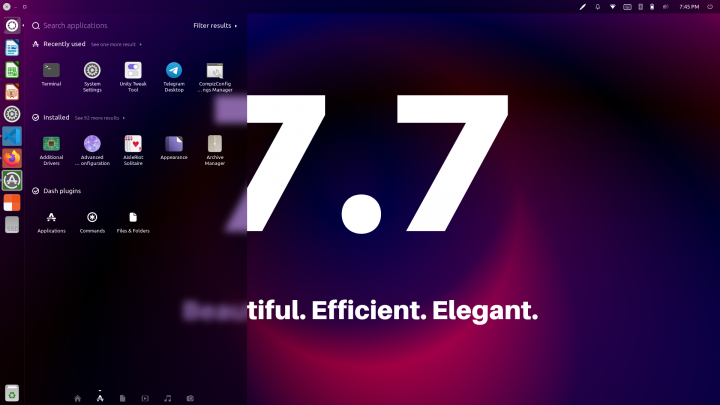
\includegraphics[width=16cm]{IKT_4_1_23@3.png}
\caption{Unity 7.7}
\end{figure}
\chapter{Fedora 38 nabídne Spiny s Budgie i Sway}
\begin{figure}[htp]
\centering

\includegraphics[width=8cm]{IKT_4_1_23@2.jpg}
\caption{Fedora Project}
\end{figure}
Před časem předložený návrh byl Fedora Engineering and Steering Committee (FESCo) schválen a počínaje příštím vydáním Fedory 38 vzniknou i oficiální Spiny s prostředími Budgie a Sway (i3 inspirované prostředí běžící na Waylandu).

Pro obě grafická rozhraní platí, že byly standardní součástí repoziářů Fedory, nyní tedy jen vzniknou předpřipravené ISO obrazy s těmito prostředími jako výchozími (podobně jako je tomu třeba pro KDE, Xfce či LXQt). Osmatřicítka je v plánu na duben tohoto roku.
\chapter{Funkční HDR na Linuxu, díky Valve}
\begin{figure}[htp]
\centering
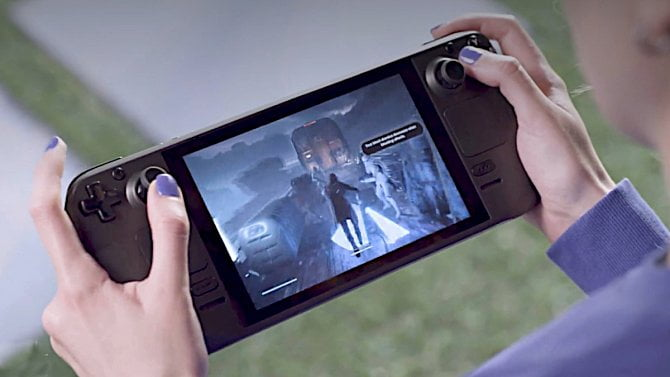
\includegraphics[width=8cm]{IKT_4_1_23@4.jpg}
\end{figure}
Valve pracuje v rámci herní platformy Steam, potažmo SteamOS pro Steam Deck, na podpoře HDR ve hrách a tudíž i obecně na Linuxu jako takovém. Jeho vývojáři nyní hlásí, že HDR je funkční, otestované minimálně na herních titulech jako Halo Infinite, Deep Rock Galactic, Death Stranding DC.

Nadále však platí, že (ne)podpora HDR je jednou z vleklých slabin linuxového grafického subsystému ve srovnání s Windows či macOS. I nynější kód je v rané, experimentální fázi vývoje, Pierre-Loup Griffais z Valve vyzdvihující nejnovější práci svého kolegy Joshe Ashtona ostatně na fotce ukazuje nastavení pro základní statický HDR systém, tedy HDR10. Doplňme také, že drtivá většina uživatelů sedí před běžnými monitory s 8bit barvami či pokud jde o 10bit model, často elektronika monitoru tuto barevnou hloubku zobrazuje pomocí techniky Frame Rate Control (tedy 8bit+FRC).
\end{document}